\section{Refined Approach}
\label{sec:refine}
The baseline approach introduced in Section~\ref{sec:basic} is not
sensitive to different senses of a term.
%In this section, we introduce
%a refined approach to address this problem.
%
%\subsection{Overview}
%
%It is necessary to identify and disambiguate senses of the terms in
%computing semantic similarity.
A simple solution is to use an
existing knowledge database containing sense labels of terms such as
the glosses in WordNet. But none of the handcrafted knowledge bases
has the sufficient data coverage. Instead we propose the following
refined approach.
%Our solution to this problem is to
%automatically determine senses in computing semantic similarity.

% cluster the concept context of a term into different groups, each
% representing a unique sense of the term. More details of this method
% and the significant refinement to the basic approach is presented in
% the next section.

Given a term, we define its {\it concept context} as the entire set of concepts that the term belongs to in Probase. We perform automatic
sense disambiguation by concept clustering.
We then prune irrelevant clusters as an optimization.
% , and we introduce a new
% similarity function based on the clustered concept contexts to compute
% similarity of two terms.
%Then, given two terms such as ``microsoft'' and ``apple'',
Finally, we define the similarity of two terms as the
highest similarity between any sense of the
first term and any sense of the second term. Next we present this approach
in details.
%Thus, we will be
%comparing the company sense of ``apple'' with ``microsoft''.
%
%The above approach has a potential challenge. Consider two terms such
%as ``music'' and ``lunch'', which do not have much
%similarity. However, each of them has a general and vague sense of~``activity'', which is captured by a small cluster of concepts. If we
%compare the two terms on this sense, we will find they have high
%similarity. To deal with this problem, we introduce an optimization
%known as cluster pruning to our algorithm. % to
% remove small clusters and vague (general) senses and thus improve the
% effectiveness of the framework.

\subsection{Concept Clustering}
To identify multiple senses of a term automatically, we first use a
k-Medoids clustering algorithm on the concept context of the term, and
then we select the center concept in each cluster to represent a sense
of this term.  Fig.~\ref{fig:clustersOfApp}(a) shows the concept
context of the term ``apple'', and Fig.~\ref{fig:clustersOfApp}(b)
shows the clustered concepts. It is clear that each cluster represents
a sense of the term.

\begin{figure}[!h]
 \centering
 \includegraphics[width=0.95\columnwidth]{clusteringResultShow.eps}
 \caption{The concept context of ``apple''}
 \label{fig:clustersOfApp}
\end{figure}

In the following, we define the distance measure and present the
clustering algorithm.

%\subsubsection{Distance Measure}

%We first introduce the lexical distance measure to identify those terms with very similar surface forms caused by the misspelling, for example, .... In terms of the edit-distance, we merge these similar concepts with a representative one and combine their entity distributions. After this preprocessing, we use the semantic distance measure function defined in Eq.~\ref{eq:semanticDist} to evaluate the distance between concepts.

\subsubsection{Clustering Algorithm}
We first define the semantic distance between two concepts $c_1$ and
$c_2$ as
\begin{equation}
\label{eq:semanticDist}
\begin{aligned}
d_{sem}(c_{1}, c_{2}) = 1-cosine(\mathcal{I}_{c_{1}}, \mathcal{I}_{c_{2}})
\end{aligned}
\end{equation}
where $\mathcal{I}_{c_i}$ represents the vector of entity distributions
of concept $c_i$ as defined in \eqnref{eq:Ic}.

Our algorithm is a modified k-Medoids clustering algorithm that
partitions concepts according to their entity distributions.  Good
initial centers are essential for the success of partitioning
clustering algorithms such as K-Means and K-Medoids. Instead of using
random initial centers, we identify good initial centers
incrementally~\cite{Moore:1991}.  The first medoid is randomly
selected among all candidate points (concepts). Then, the point that has the maximum of the minimum of the distances from each of the existing medoids is selected to be the next medoid, namely the point satisfying \eqnref{eq:initMedoid}, where $c_j$ indicates the $j^{th}$ point in the candidate points, $m_i$ indicates the $i^{th}$ medoid in existing medoids.
\begin{equation}
m = \max_{c_j}\{\min_{i}\{d_{sem}(m_i,c_j)\}\}
\label{eq:initMedoid}
\end{equation}
%Then, the point that
%has the maximum distance to existing medoids % (defined by the minimum
%% distance to any of the existing medoid)
%is selected to be the next medoid.
This process continues until we
have chosen $k$ medoids at iteration 0: $M^{0} = \{m_{1}^{0}, ...,
m_{k}^{0}\}$.

%How to update after once iteration (how to determine the centroid)?
With \emph{k} medoids in the $t^{th}$ iteration, we assign each
candidate concept $c_{i} \in C$ to its closest medoid $m^{*}\in M^{t}
= \{m_{1}^{t}, ..., m_{k}^{t}\}$, namely, a medoid $m^{*}$ with the
minimum semantic distance from $c_{i}$:
\begin{equation}
\label{eq:newCentroid}
m^* = \argmin_{m_{j}^{t}\in M^{t}}d_{sem}(c_{i}, m_{j}^{t})
\end{equation}
When we assign all candidate concepts to the corresponding clusters,
we can update the medoid with the most centrally located concept in
each cluster.  To find such a center concept, we first compute the
average distance of a cluster $C_{i}$ in terms of the semantic
distance in \eqnref{eq:semanticDist} as
\begin{equation}
\label{eq:update}
m_i^{t+1} = \argmin_{c_{y}\in C_{i}}\left(\sum_{c_x\in C_{i}}\frac{d_{sem}(c_{x},c_y)}{|C_{i}|}\right)
\end{equation}
%Thus, we find the new centroid $m^{t+1}_{i}$ in the $(t + 1)^{th}$ iteration
%whose the average semantic distance is the minimum one.
The clustering process iterates until an objective function converges.
%What should be the objective function of clustering?
The objective function is to find \emph{W} and \emph{M} that minimize
\begin{equation}
\label{eq:objectiveFun}
\begin{aligned}
F(W,M)=\sum^{k}_{i=1}\sum^{n}_{j=1}w_{ij}d_{sem}(m_{i},c_{j})
\end{aligned}
\end{equation}
where \textit{w}$_{ij}\in$\{0, 1\},
$\sum^{k}_{i=1}w_{ij}=1$, 0$<\sum^{n}_{j=1}w_{ij}<n$,
$k~ (<n)$ is a known number of centers, \emph{n} is the count of objects (concepts) to cluster.
$W = [w_{ij}]$ is a
$k \times n$ binary matrix, $M=[m_{1}, \ldots, m_{k}]$ is a set of cluster medoids
and $m_i$ is the $i^{th}$ cluster medoid.

%The matrices \emph{W} and \emph{M} are calculated according to the following two theorems provided in \cite{Ng:2007}.
We use \eqnref{eq:update} to calculate the medoid set $M$.
When $M$ is computed, to minimize $F(W, M)$, $W$ is given by
\begin{equation}
\label{eq:weight}
\noindent {w_{ij} = \left\{
\begin{aligned}
1 & \hspace*{5pt} \mbox{if}~ d_{sem}(m_{i},c_{j}) < d_{sem}(m_{h},c_{j})\\
 & \hspace*{25pt} (1 \leq h \leq k,~h \neq i)\\
0 & \hspace*{5pt} \mbox{otherwise}
\end{aligned}
\right.}
\end{equation}
The convergence condition is that $F(W^{t}, M^{t+1})- F(W^{t}, M^{t})$
is less than a threshold $\delta$ (e.g., $10^{-5}$). The minimization
of \emph{F} in \eqnref{eq:objectiveFun} with the above constraints
forms a class of constrained nonlinear optimization problems whose
solutions are unknown. The usual method to optimize $F$ is to use a
partial optimization for $M$ and $W$ as shown in Algorithm
\ref{alg:conceptClustering}.

%\makeatletter\def\@captype{algorithm}\makeatother
\renewcommand\algorithmicrequire{\textbf{Input:}}
\renewcommand\algorithmicensure {\textbf{Output:}}
\begin{algorithm}[th]
%\begin{center}
\caption{Concept Clustering}
\label{alg:conceptClustering}
%\caption{Context-based semantic cleaning approach} \label{algo_minball}
\begin{algorithmic}[1]
\REQUIRE $C=\{c_{1}, ...c_{j},...\}$: the concept set;\\
~~~~~~$k$: the number of initial medoids;\\
~~~~~~$T$: the maximum iteration count; \\
~~~~~~$\Gamma_{isA}$: the semantic network of isA relationship;\\
\ENSURE \emph{k} clusters $\{C_{1}, ..., C_{k}\}$;
\STATE Initialize the iteration time \emph{t} = 0;
\STATE Generate an initial medoid set $M^{t}=[m_{1}^{t}, m_{2}^{t}, \cdots, m_{k}^{t}]$ incrementally;
\STATE Assign each concept $c_{i}$ to a cluster $C^{*}$ with a medoid $m^{*}$ satisfying
\eqnref{eq:newCentroid};
\STATE Update the weight matrix $W^{t}$ in \eqnref{eq:weight} to make sure $F(W^t, M^t)$ is minimum;
\STATE Update cluster medoids in $M^{t+1}$ with the most centrally located point in each cluster corresponding to \eqnref{eq:update};
\STATE Calculate $F(W^t, M^{t+1})$ in \eqnref{eq:objectiveFun};
\IF {$F(W^t, M^{t+1})$-$F(W^t, M^t)$ $ > \delta$ and \emph{t} < \emph{T}}
\STATE Let \emph{t} = \emph{t}+1 and go to Step 3;
\ENDIF
\STATE return clusters $\{C_{1}, ..., C_{k}\}$;
\end{algorithmic}
%\end{center}
\end{algorithm}

\subsubsection{Offline Concept Clustering}
%We first analyze the computational complexity in our concept clustering approach.
The k-Medoids clustering algorithm has a time complexity of $O(kn^{2})$,
where $k$ is the number of centers and $n$ is the number of objects (concepts)
to cluster.
%In this case, given a pair of terms, if we install clustering after we collect the concept contexts (we call this processing as the online clustering), it is hard to apply into measuring the semantic similarity of millions pairs even if online clustering for each pair consumes only a few seconds. More precisely, suppose we have 1 million pairs and the time overhead of online clustering for each pair is only 1 second, we will spend 11.57 days at least on the measuring of semantic similarity of all pairs.
This is not acceptable if the online application requires the computation of
many pairs of terms at the same time. To improve the efficiency, we cluster all concepts
in the semantic network offline, and then during online calculation,
each concept in a term's context can be quickly mapped to an offline cluster
which acts as synset, and this effectively reduces the online clustering
complexity to $O(n)$.
%we only need to find the cluster information directly after collecting
%the concept contexts of a pair.
%In this case, the time overhead of clustering the concept context
%of each term can be reduced to 5 milliseconds on average.
%We call this processing as the offline clustering.

\begin{figure}[th]
%\makeatletter\def\@captype{figure}\makeatother
 \centerline{
 \includegraphics[width=0.6\columnwidth]{bipartition-small.eps}}
\caption{A concept-entity bipartite graph} \label{fig:bipartition}
\end{figure}

%There are some challenges in the clustering all concepts
%in the semantic network.
To cluster the concepts in the semantic network,
we use the entity distributions to represent the concepts and
evaluate their similarities by \eqnref{eq:semanticDist}.
According to the isA relationships between concepts and entities in
$\Gamma_{isA}$, we can construct a bipartite graph
between concepts and entities (Fig.~\ref{fig:bipartition})
and cluster the concepts based on this graph.
The basic idea is that if two concepts share many entities,
they are similar to each other. From this concept-entity bipartite,
we represent each concept $c_i$ as an L2-normalized vector as shown
in \eqnref{eq:Ic}, where each dimension corresponds
to an entity in the graph.

On the surface, there are two challenges in clustering concepts
on the bipartite graph. First, the concept nodes in this bipartite are large,
as $\Gamma_{isA}$ consists of more than 2.7 million unique concepts.
%Therefore, the clustering algorithm must be efficient and scalable
%to handle large data sets.
Second, the dimension $\mathcal{I}_c$ is also large, with
over 5.5 million unique entities in $\Gamma_{isA}$.
%the data set is hence of extremely high dimensionality.
%Therefore, the clustering algorithm must tackle the
%``curse of dimensionality''.
Fortunately, in reality, the graph is very sparse.
%To overcome the above problems and find the closest cluster fast in our algorithm, we observe that the concepts in $\Gamma_{isA}$ are very sparse.
For example, a concept is connected with an average
number of 5.72 entities in $\Gamma_{isA}$. Each entity is also connected to a couple of concepts on average.
%The average degree of entities nodes is only 2.58.
Therefore, for a concept $c$, the average size of $S_c$,
the set of concepts which share at least
one entity with $c$, is small.
%is only $5.72\times (2.58-1) = 9.04$. Intuitively,
%for any cluster $C$, if $C \cap S_c = \emptyset$, \emph{C} cannot be close to $c$ since the distance of any member of \emph{C} to $c$ is 1, which is the farthest distance calculated according to \eqnref{eq:semanticDist}.
To find the closest cluster to $c$,
we only need to check the clusters which contain at
least one concept in $S_c$. Since each concept belongs to only one
cluster in our method, the average number of clusters to be checked is small.
%no more than 9.04.
We thus use an efficient dimension array data structure\cite{Cao:2008}
to facilitate the above checks.
Furthermore, edges in the graph with low weights (i.e., low typicality scores)
are likely to be noises and can be ignored. This can further simplify the graph
and speed up the clustering.
%be formed due to some noisy isA relationships especially for lower co-occurrences of concepts and entities. Thus, we aim to prune these noisy concepts and entities without degrading the quality of clusters. More precisely, let $w_{ij}$ be the weight (namely the typicality score $p(e_j|c_i)$) between $c_i$ and $e_j$, let $w_i$ be the sum
%of the weights of all entities that $c_i$ contains, i.e.,
%$w_i =\sum_j w_{ij}$. We can prune an edge connecting $c_i$ and $e_j$ if the absolute
%weight the relative weight $w_{ij}/w_i < \alpha$, in our experiments,
%we set $\alpha =$ 0.001.
%After the pruning process, our clustering algorithm can finish in 15 hours when clustering 2.7 million concepts in $\Gamma_{isA}$ running on a PC of 4 GB main memory.
%


%%% Local Variables:
%%% mode: latex
%%% TeX-master: "paper"
%%% End:


\subsection{The Max-Max Similarity Function}
%We now give a general framework of measuring the semantic similarity between
%terms using the concept clustering. As shown in Algorithm \ref{alg:refined},
%our clustering-based approach also has three steps similar to the basic approach.
%% That is, we first judge the type of terms. Second, we represent the semantic contexts of each term according to its type, that is, modeling a probability distribution over contexts. Third, we compare how similar these two discrete probability distributions are by encoding them as vectors and computing the cosine between the vectors.
%The difference is that we add the clustering in Algorithm \ref{alg:conceptClustering}
%on all concept contexts of terms for their possible senses,
%and then evaluate the semantic similarity by comparing these
%concept-cluster contexts. We will give the details on the
%concept-cluster-based similarity evaluation in the following section.
%
%
%\subsubsection{Context Comparison}
In the basic approach, we compute the similarity of two terms
by the cosine similarity between their contexts. In the
refined approach, we use a new similarity function known as {\em max-max similarity}
which is useful in identifying rare senses of terms with small sized clusters.
%We formalize the concept cluster-based context comparison method as follows.
Let $K=\{K_1,K_2,...,K_k\}$ be clusters of all concepts in $\Gamma_{isA}$,
$C_{t_1}$ and $C_{t_2}$ be the sets of concepts that two terms belong to
respectively.
 %{\color{red} We can represent them as $C_p = \{c_{1}, c_{2}, ..., c_{|C_p|}\}$ ($1\leq p\leq k$), $C^{t_1} = \{c^{t_1}_{1},c^{t_1}_{2},...,c^{t_1}_{m}\}$ and $C^{t_2} = \{c^{t_2}_{1},c^{t_2}_{2},...,c^{t_2}_{n}\}$, where $c_{q}$ ($1\leq q\leq |C_p|$), $c^{t_1}_{i}$ ($1\leq i\leq m$) and $c^{t_1}_{j}$ ($1\leq j\leq j$) indicate a concept in $\Gamma_{isA}$, $C^{t_1}$ and $C^{t_2}$ respectively, meanwhile, $C_p$, $C^{t_1}$ and $C^{t_2}$ satisfy $C_p \subset \Gamma_{isA}$, $C^{t_1}\subset \Gamma_{isA}$ and $C^{t_2}\subset \Gamma_{isA}$ respectively. According to the cluster information in $C$,
%we divide all concepts in $C^{t_1}$ and $C^{t_2}$ into small clusters
%$C^{t_1}=\{C^{t_1}_{1},..., C^{t_1}_{m}\}$ and
%$C^{t_2}=\{C^{t_2}_{1},..., C^{t_2}_{n}\}$ by
%comparing each concept $c^{t_1}_{i}$ in $C^{t_1}$ and each concept $c^{t_2}_{j}$ in $C^{t_2}$ with $c_{q}$ in $C_p$ respectively. If $c^{t_1}_{i} == c_{q}$ or $c^{t_2}_{j}== c_{q}$, we can label $c^{t_1}_{i}$ or $c^{t_2}_{j}$ by the cluster of $C_p$.}
According to the cluster information in $K$, we can get the clusters in $C_{t_1}$ and $C_{t_2}$, namely $K_{t_1}$ and $K_{t_2}$ as follows.
\[K_{t_1} = \{ x | x = K_i \cap sup(t_1),
\forall K_i \in K \land x \ne \emptyset\}\]
and
\[K_{t_2} = \{ y| y = K_i \cap sup(t_2),
\forall K_i \in K \land y \ne \emptyset\},\]
where \[sup(t_i) = \{c | \langle c, t_i \rangle \in \Gamma_{isA}\}.\]
%In this case, we can represent $C_{t_1}^{x}$ and $C_{t_2}^{y}$ as $C_{t_1}^{x} = \{c^{t_1}_1, c^{t_1}_2, ..., c^{t_1}_p\}$
%and $C_{t_2}^{y} = \{c^{t_2}_1, c^{t_2}_2, ..., c^{t_1}_q\}$ respectively.
%The corresponding value vectors of $C^{t_1}_{x}$ and $C^{t_2}_{y}$ can be represented by $\mathcal{I}_{t_1}^{x} = \langle p(c^{t_1}_1|t_1),\cdots,p(c^{t_1}_p|t_1) \rangle$ and $\mathcal{I}_{t_2}^{y} = \langle p(c^{t_2}_1|t_2),\cdots,p(c^{t_2}_q|t_2) \rangle$ respectively.
We then compute the similarity between the contexts of each cluster pair
and get the semantic similarity between two terms as:
\begin{equation}
\begin{aligned}
sim(T(t_{1}), T(t_{2})) = \max_{x \in K_{t_1}, y \in K_{t_2}}\{cosine(x, y)\}
\label{eq:clusterCosine}
\end{aligned}
\end{equation}
%~~~~~~~~~~~~~= \max_{x, y}\{cosine(\mathcal{I}_{t_1}^{x}, \mathcal{I}_{t_2}^{y})\}
The corresponding value vector of \emph{x} (or \emph{y}) indicates the set of typicality scores for $t_1$ (or $t_2$) and each concept in $sup(t_1)$ (or $sup(t_2)$).

With all concepts clustered offline and the new similarity function
based on concept clusters, the refined algorithm is given in
Algorithm \ref{alg:refined}.
%
% \begin{table}[!h]
% \centering
% \caption{Concept clusters of a pairwise term Microsoft and Apple}% (extracted using Hearst patterns)}
% \label{tab:microsoft-apple-clusters}
% \begin{tabular}{|p{2pt}|l|c|p{2pt}|l|c|}\hline
%  & concepts &  &  & concepts & \\
% id & of Microsoft & weight & id & of Apple & weight\\\hline
% 1 &company    &0.3738 &1  &fruit  &0.2952\\
% 1 &u.s. company   &0.0349 &1  &seasonal fruit &0.0826\\
% 1 &client &0.0256 &1  &tree fruit &0.0048\\
% 1 &large company  &0.0227 &1  &fresh fruit    &0.0389\\
% 1 &software giant &0.0217 &1  &juice  &0.0067\\
%   &international-&    &   &   &\\
% 1 &company    &0.0207 &1  &fruit juice    &0.0065\\
%   &technology-    &   &   &   &\\
% 1 &company    &0.0145 &1  &dried fruit    &0.0051\\
% 1 &software company   &0.0141 &2  &company    &0.1239\\
% 1 &big company    &0.0125 &2  &manufacturer   &0.0100\\
% 1 &giant  &0.0123 &2  &competitor &0.0077\\
% 1 &player &0.0112 &2  &large company  &0.0048\\
% 1 &software vendor    &0.0095 &3  &food   &0.0612\\
% 1 &competitor &0.0086 &3  &snack  &0.0054\\
% 1 &partner    &0.0082 &3  &healthy snack  &0.0052\\
% 1 &manufacturer   &0.0071 &4  &fruit tree &0.0223\\
% 1 &industry giant &0.0068 &4  &tree   &0.0083\\
% 1 &big player &0.0063 &5  &brand  &0.0216\\
% 2 &organization   &0.0217 &6  &crop   &0.0147\\
% 3 &provider   &0.0184 &7  &flavor &0.0121\\
% 4 &industry leader    &0.0184 &8  &product    &0.0067\\
% \hline
% \end{tabular}
% \end{table}
%
%For example, Table~\ref{tab:microsoft-apple-clusters} shows the top 20 concepts of the entity pair $<microsoft,~apple>$, according to the cluster information in $C$, we can get the clusters that each concept belongs to. In terms of Eq.~\ref{eq:clusterCosine}, we can get the maximum similarity score of this pair, namely the cosine score by comparing the context of Microsoft in the $1^{st}$ cluster with that of Apple in the $2^{nd}$ cluster. In this case, the similarity score between Microsoft and Apple is improved from 0.378 in Eq.~\ref{eq:cosine} to 0.994 in Eq.~\ref{eq:clusterCosine}.
%
%\makeatletter\def\@captype{algorithm}\makeatother
%\KZ{Is it possible to simplify this algo? The structure looks the same as
%Algo 1.} \LP{revised}

\renewcommand\algorithmicrequire{\textbf{Input:}}
\renewcommand\algorithmicensure {\textbf{Output:}}
\begin{algorithm}[th]
%\begin{center}
\caption{Refined Approach}
\label{alg:refined}
\begin{algorithmic}[1]
\REQUIRE \pair{t_1}{t_2}: a pair of terms;\\
~~~~~~$\Gamma_{isA}$: the semantic network of isA relationship;\\
~~~~~~$\Gamma_{ssyn}$: the synset data set in $\Gamma_{isA}$;\\
~~~~~~$\Gamma_{cluster}$: clusters of all concepts in $\Gamma_{isA}$;
\ENSURE a similarity score of \pair{t_1}{t_2};
\STATE Install the synset checking and type checking as Steps 1-4 in Algorithm \ref{alg:baseline};
\IF {\pair{t_1}{t_2} is a concept pair}
\STATE return $sim(\mathcal{I}_c^{t_1}, \mathcal{I}_c^{t_2})$ as Steps 6-7 in Algorithm \ref{alg:baseline};
\ENDIF
\IF {\pair{t_1}{t_2} is an entity pair}
\STATE $sim_1\leftarrow sim(\mathcal{I}_e^{t_1}, \mathcal{I}_e^{t_2})$ as Steps 10-11 in Algorithm \ref{alg:baseline};
\STATE Find clusters of contexts $K_{t_1}$ and $K_{t_2}$ from $\Gamma_{cluster}$;% and prune the cluster sets;
\STATE $sim_2\leftarrow sim(K_{t_1}, K_{t_2})$ computed in \eqnref{eq:clusterCosine};
\STATE return $max(sim_1, sim_2)$;
\ENDIF
\IF {\pair{t_1}{t_2} is a concept-entity pair}
\STATE Collect all concepts of the entity term $t_i$ from $\Gamma_{isA}$ as the context $C_{t_i} (i\in\{1, 2\})$;
\STATE Find clusters of contexts $K_{t_i}$ from $\Gamma_{cluster}$;% and prune the cluster sets;
\FOR {each cluster $x$ in $K_{t_i}$}
\STATE Select top $k$ concepts to represent $t_i$, namely $C{^{k}_{x}}=\{c_y|c_y \neq t_j,c_y\in x, 1\leq y \leq k\}$;
\FOR {each concept $c_y$ in $C{^{k}_{x}}$}
\STATE $sim_{c_y}\leftarrow$ get the semantic similarity between $c_y$ and $t_j$ by repeating this algorithm iteratively;
\ENDFOR
\STATE $sim_x\leftarrow max_{c_y\in C{^{k}_{x}}}\{sim_{c_y}\}$;
\ENDFOR
\STATE return $max\{sim_{x}|x\in K_{t_i}\}$;
\ENDIF
\end{algorithmic}
%\end{center}
\end{algorithm}


\subsection{Optimization by Cluster Pruning}
%We now discuss the advantage and disadvantage using the clustering-based approach for measuring semantic similarity between terms.
%Table~\ref{tab:examples} compares the semantic similarity scores of 9 pairs predicted in Eq.~\ref{eq:clusterCosine} and Eq.~\ref{eq:cosine}. From the experimental results, we can see that comparing the baseline approach using Eq.~\ref{eq:cosine}, our clustering-based approach using Eq.~\ref{eq:clusterCosine} ac
%tually improve the semantic similarity of pairs, such as $<Apple,~Microsoft>$, $<Orange,~Red>$ and $<Microsoft, GE>$ those with ambiguous terms whose data d
%istributions of senses hidden in contexts are skewed. However, it also improves the similarity score of dissimilar pairs like $<lunch,~music>$. This is cause by the following reasons.
The cluster-based refined approach improves the quality of similarity remarkably from
the basic algorithm. But there are two problems. First, the max-max similarity function tends to boost the probability of picking
a less dominant sense of a term because it is easier for
small clusters to look similar
by the cosine similarity and hence dominate the max-max similarity score. However, many small clusters in $C$ are usually noises. This leads to incorrect
similarity results.
%
%First, there are some noisy concepts in the tail of the concept context given a term, which lead to many small sized clusters formed when using the offline
%clustering method.
%For example, as shown in Table~\ref{tab:microsoft-apple-clusters}, there are small clusters like crop and flavor in the top 20 concepts of Apple, which does
% not accurately represent a sense of Apple.
Second, with the current concept clustering algorithm, some terms can have both a general sense and a more specific sense. For example, the term
``lunch'' has a specific sense called ``dish'' and a more general (and also vague) sense called ``activity''. We know ``activity'' is  more
general because it is a super-concept of ``dish'' in $\Gamma_{isA}$. Such general senses pose problems because they make almost unrelated terms
similar. For example, the term ``music'' also has the ``activity'' sense and thus is deemed similar to ``lunch''.
%
%some term we can get some general (vague) senses except of specific senses when clustering the concept context, because we clustering all concepts flatly. For
% example, considering the senses of Music and Lunch as shown in Table~\ref{tab:sensesOfSamples}, we call the Activity sense as a vague sense and the dish and multimedia senses as specific ones. This is because the former is a super concept of the latter according to the isA relationships in $\Gamma_{isA}$, whose importance as the sense of the term is less than the latter.
%

To overcome these problems, we adopt an optimization technique called
{\em cluster pruning} after concept clustering.
First, to reduce the negative impact from noisy clusters,
we prune away those clusters with only one member or with very small combined weight.
% the weight is lower than the threshold $\tau$ (e.g., 0.01).
%We use the normalized sum typicality of scores for the term \emph{e}
%and its concept $c_i$ in a cluster $C_x$ as the weight of the current cluster.
The weights of clusters are computed below. Let the concept clusters of the term \emph{t} be $K^t = \{x_1,...,x_m\}$,
the weight of each cluster $x_i$ is $w_i/\sum_{i}w_i$, where
$w_i = \sum_{c_j\in x_i}p(c_j|t)$ and $1 \leq i \leq m$.
%In this processing, we can get more accurate senses for each terms. For example, Table~\ref{tab:sensesOfSamples} summarizes main senses of ambiguous terms in Table~\ref{tab:examples} according to the cluster centers and their weights.
Second, to avoid the impact from the vague senses, we prune the clusters whose senses are super-concepts of other senses according to the isA
relationships in $\Gamma_{isA}$. For example, Figure~\ref{fig:clusters-given-a-pair} shows a hierarchical isA relationships of senses after
clustering concept contexts of two terms ``lunch'' and ``music''. Because the senses ``Activity'', ``Cost'', ``Interest'' and ``Art'' are the
super-concepts of the senses ``Dish'' and ``Multimedia'', we only keep specific senses like ``Dish'' and ``Multimedia'' and remove the rest.
%then we compare their contexts in the clusters in Eq.~\ref{eq:clusterCosine}.
%Finally, we can get the similarity between Lunch and Music,
%which is reduced to \textbf{0.012}.

%\begin{table}[!t]
%\centering
%\caption{Main senses of sampling terms}
%\label{tab:sensesOfSamples}
%\begin{tabular}{|c|c|c|c|} \hline
%entity &id &   senses  &weight\\\hline
%   &1  &Fruit & 0.792\\
%Apple  &2  &Company &0.138\\
%   &3  &Fruit Tree & 0.080\\\hline
%   &1  &Fruit & 0.457\\
%Orange &2  &Color &0.447\\
%   &3  &Company&0.014\\\hline
%GE &1  &Company & 0.606\\
%   & 2 &Material&0.394\\\hline
%   &1  &Interest &0.518\\
%Music  &2  &Multimedia&0.201\\
%   &3  &Activity & 0.196\\
%   &4  &Art&0.085\\\hline
%   &1  &Dish &0.501\\
%Music  &2  &Activity&0.251\\
%   &3  &Cost&0.248\\\hline
%Pear   &1  &Fruit & 0.824\\
%   &2  &Fruit Tree & 0.097\\\hline
%Microsoft  &1  &Company &0.895\\\hline
%\end{tabular}
%\end{table}

\begin{figure}[th]
 \centerline{
 \includegraphics[width=0.9\columnwidth]{clusters-given-a-pair.eps}}
\caption{Illustration to vague and specific senses of terms lunch and music} \label{fig:clusters-given-a-pair}
\end{figure}



%%% Local Variables:
%%% mode: latex
%%% TeX-master: "paper"
%%% End:
